\begin{frame}
  \frametitle{Motivation}
  \begin{block}{Why model Pyroprocessing?}
  	\begin{itemize}
  		\item Safeguard by design.
  		\item Future fuel cycles.
  	\end{itemize}
  \end{block}
 \begin{block}{What is the goal?}
 	PyRe will be used to answer the following questions
 	\begin{itemize}
 		\item What is the effect of introducing pyroprocessing plants in the fuel cycle?
 		\item How do various facility designs affect throughput and efficiency?
 		\item Where in a pyroprocessing plant will monitoring most 
 		effectively detect material diversion?
 	\end{itemize}
\end{block}
The first two can be directly answered by the archetype. The third requires data analysis via
diversion algorithms.	
\end{frame}

\begin{frame}
\frametitle{Cyclus}
\begin{block}{What is Cyclus?}
	Cyclus is a modular agent based fuel cycle simulator for tracking commodity transactions
	between facilities.
\end{block}
\begin{figure}
	\centering
	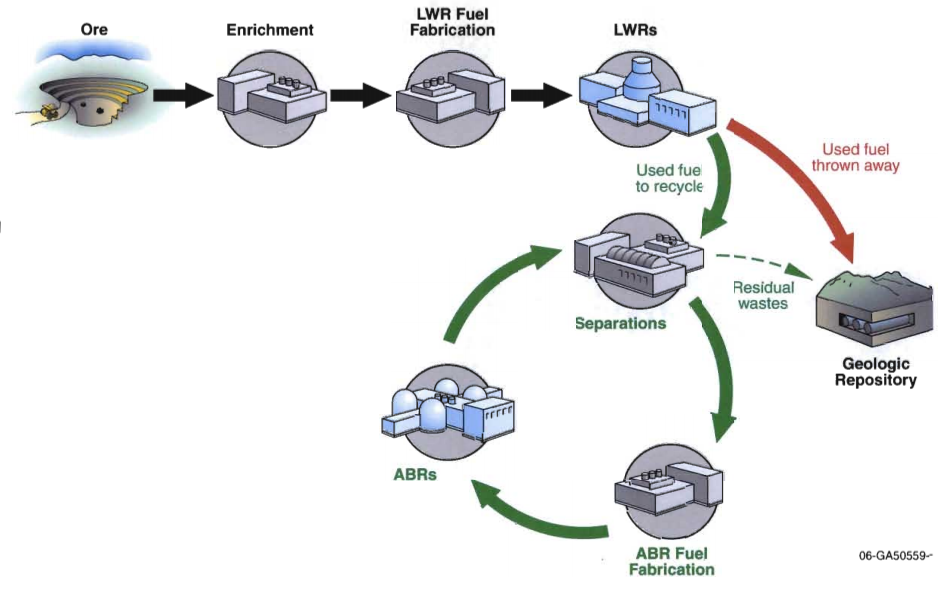
\includegraphics[width=0.7\linewidth]{lanl-fuel-cycle.png}
\end{figure}
\end{frame}

\begin{frame}
\frametitle{Why Cyclus?}
Cyclus allows the construction of specific scenarios through the addition of archetypes. These archetypes are
modular and the transactions can be tracked.
	\begin{figure}
		\centering
		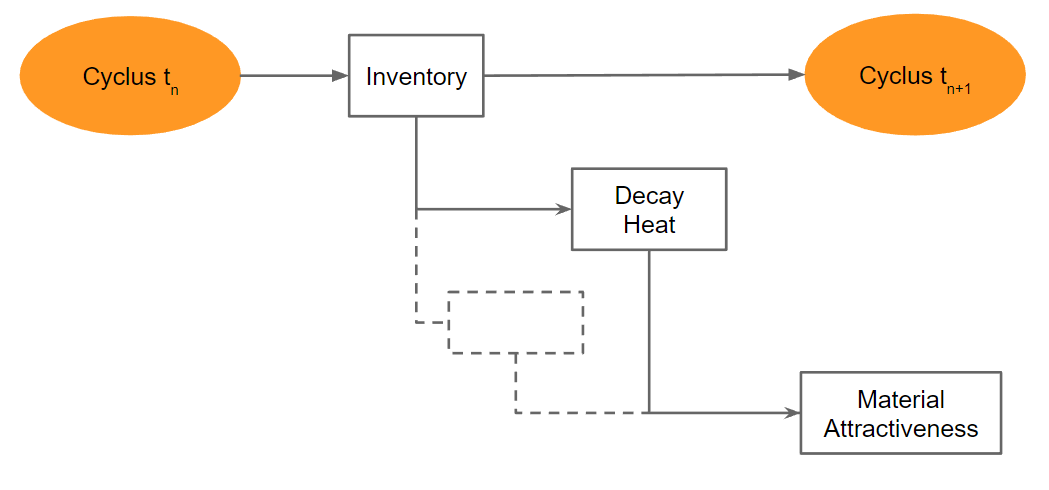
\includegraphics[width=0.9\linewidth]{diversion1}
		\caption{Diversion detection methods within Cyclus.}
		\label{fig:diversion}
	\end{figure}
\end{frame}
